\documentclass[a4paper]{article}

\usepackage[T1]{fontenc}
\usepackage[utf8]{inputenc}

\usepackage{float}
\usepackage{amsmath}
\usepackage{graphicx}
\usepackage{csquotes}
\usepackage{dirtytalk}
\usepackage{hyperref}
\usepackage{xcolor}
\usepackage{listings}
\lstset{
  basicstyle=\ttfamily,
  columns=fullflexible,
  frame=single,
  breaklines=true,
  postbreak=\mbox{\textcolor{red}{$\hookrightarrow$}\space},
}
\newcommand\todo[1]{\textcolor{red}{TODO: #1}}

\title{REI105M\\Forritun Ofurtölva\\Assignment 2}
\author{Þór Tómasarson}

\begin{document}
\maketitle


\begin{enumerate}
    \item
    Understanding shared memory programming with OpenMP
    \begin{enumerate}
    \item
    \textit{OpenMP Hello World}

    The \textbf{OpenMP Hello World} program was executed on the cluster both with 4 nodes and then with 8 nodes. The sbatch script used along with it’s execution output for 4 nodes can be seen in Figure~\ref{fig:helloworld}.
    
    \begin{figure}[H]
        \centering
        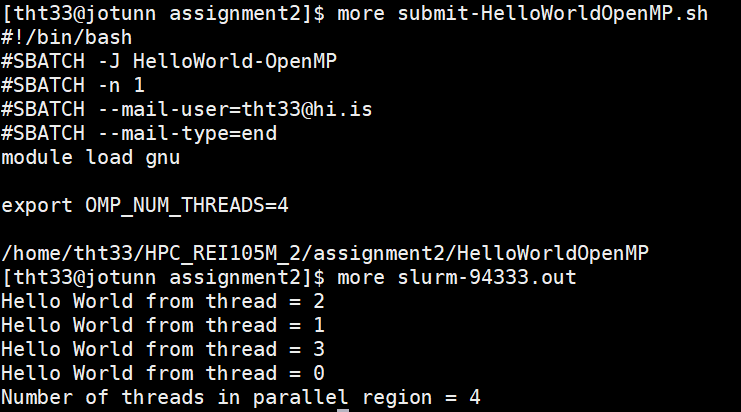
\includegraphics[scale=0.7]{images/HelloWorld}
        \caption{\label{fig:helloworld}\textbf{OpenMP Hello World} program on 4 nodes}
    \end{figure}

    \item
    \textit{OpenMP loop compiler directive}
    
    The \textbf{Loop OpenMP} program adds up the contents from two arrays into one, $a[i] = b[i] + c[i]$. Where the arrays $b$ and $c$ are defined as $b[i] = i$ and $c[i] = i*i$. Executions with different sizes for the arrays where tested out along with different number of parallel threads. The execution time varied allot, for example when the array sizes where set to 32,000 with 3 threads the execution time was $\approx1.5$ sec but with 30 threads the execution time was $\approx 1.0$ sec (both executions where writing out to IO).

    The output for the program execution with array sizes of 10 and 4 threads can be seen in Figure~\ref{fig:LoopOpenMP}. The output shows the elapsed time since start of program at each written line in the output, as can be seen there the outputs do not appear in correct time order. The behavior is caused by the race condition to the IO for all the threads running.

    \begin{figure}[H]
        \centering
        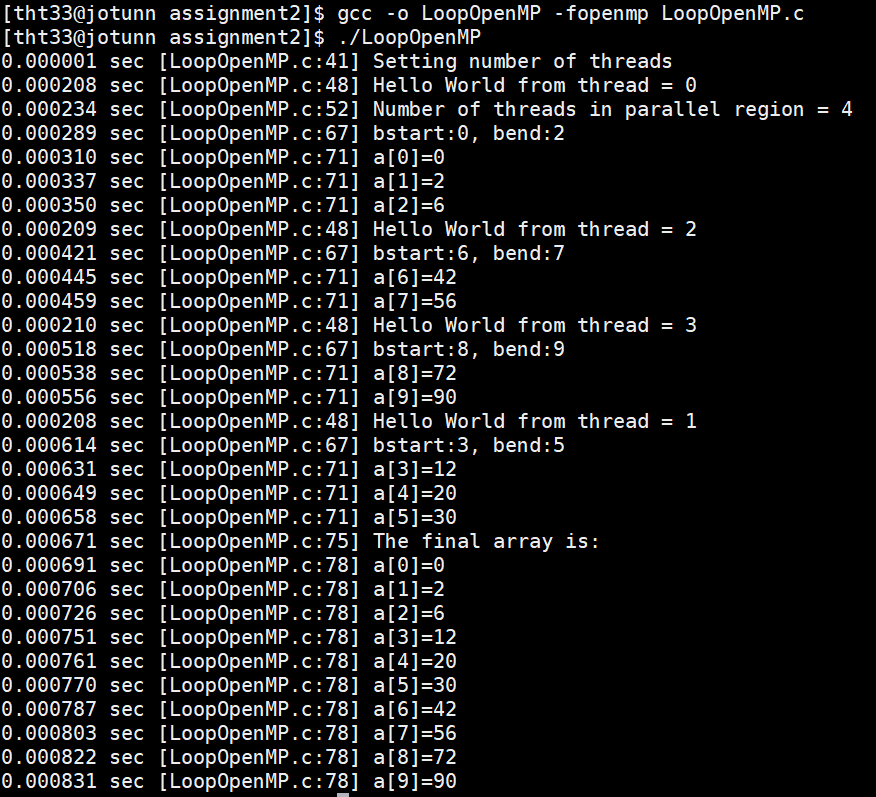
\includegraphics[scale=0.7]{images/LoopOpenMP_4}
        \caption{\label{fig:LoopOpenMP}Output from execution of the \textbf{OpenMP Loop} program}
    \end{figure}

    \end{enumerate}

    \item
    Understanding concurrency with MPI
    \begin{enumerate}
    \item
    \textit{Elevator}
    
    ...

    \begin{figure}[H]
        \centering
        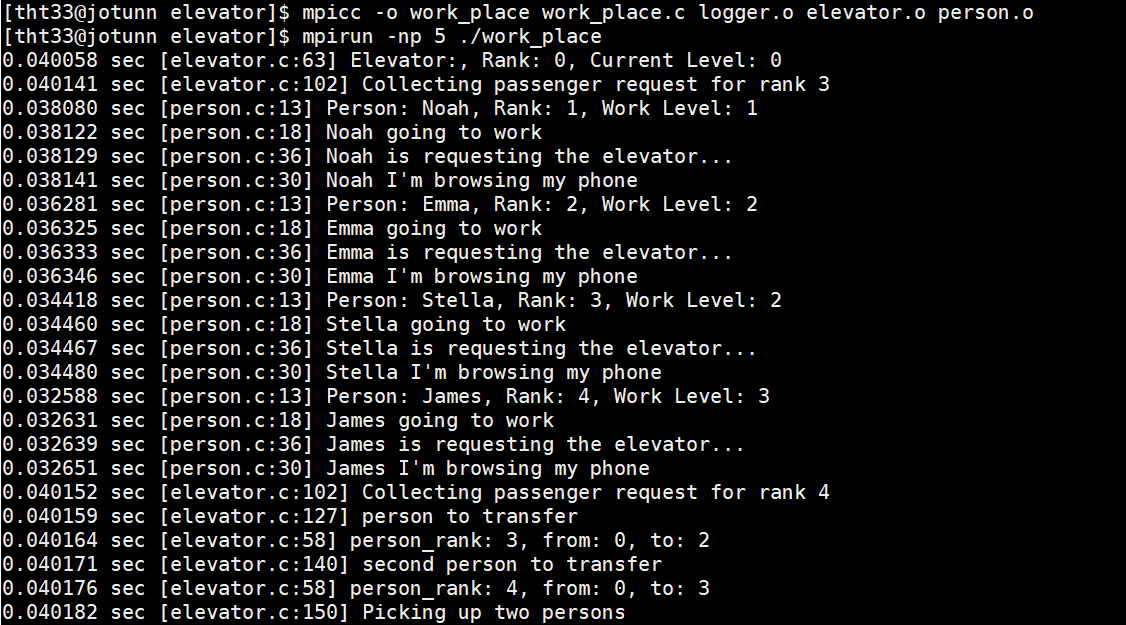
\includegraphics[scale=0.7]{images/mixed_logging}
        \caption{Part of output from execution of the \textbf{Work Elevator} program with 4 persons}
    \end{figure}

    \end{enumerate}
\end{enumerate}

\end{document}
